\documentclass[tikz,border=8pt]{standalone}
\usepackage{amsmath,amssymb}
\usetikzlibrary{arrows.meta,calc,decorations.markings}

\begin{document}
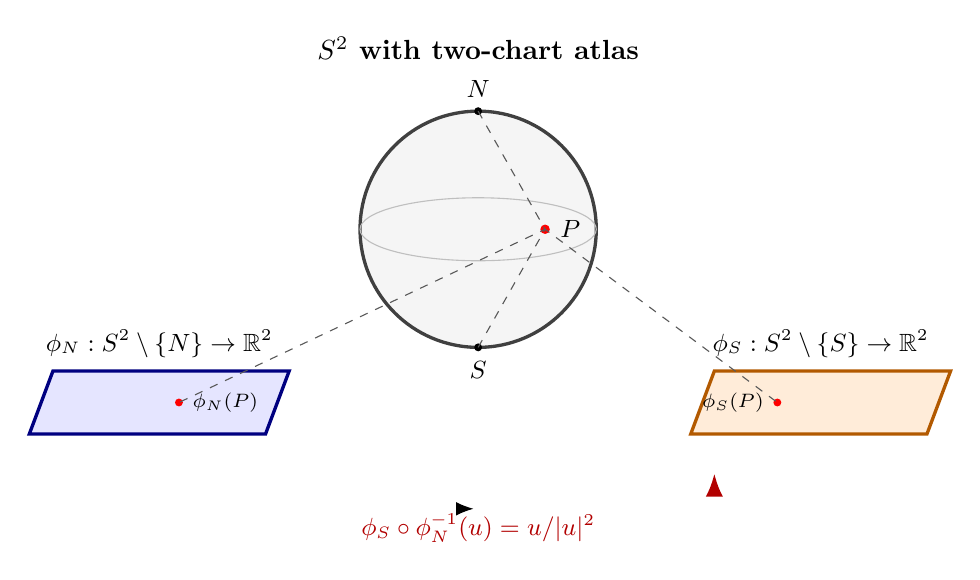
\begin{tikzpicture}[>=Latex]

  % Title
  \node[font=\bfseries] at (0, 4.0) {$S^2$ with two-chart atlas};

  % Sphere
  \draw[very thick, gray!50!black, fill=gray!8] (0, 1.7) circle (1.5);
  \draw[gray!50, thin] (0, 1.7) ellipse (1.5 and 0.4);

  % North pole and South pole
  \fill[black] (0, 3.2) circle (0.05);
  \node[font=\small, anchor=south] at (0, 3.25) {$N$};
  \fill[black] (0, 0.2) circle (0.05);
  \node[font=\small, anchor=north] at (0, 0.15) {$S$};

  % Point P on sphere (off-center)
  \fill[red] (0.85, 1.7) circle (0.06);
  \node[font=\small, anchor=west] at (0.92, 1.7) {$P$};

  % Left chart (north): R^2 plane
  \begin{scope}[xshift=-4.2cm, yshift=-0.3cm]
    \fill[blue!10] (-1.5, -0.6) -- (1.5, -0.6) -- (1.8, 0.2) -- (-1.2, 0.2) -- cycle;
    \draw[very thick, blue!50!black] (-1.5, -0.6) -- (1.5, -0.6) -- (1.8, 0.2) -- (-1.2, 0.2) -- cycle;
    \node[font=\small, anchor=south] at (0.15, 0.25) {$\phi_N: S^2\setminus\{N\}\to\mathbb R^2$};
    \fill[red] (0.4, -0.2) circle (0.05);
    \node[font=\scriptsize, anchor=west] at (0.45, -0.2) {$\phi_N(P)$};
  \end{scope}

  % Right chart (south): R^2 plane
  \begin{scope}[xshift=4.2cm, yshift=-0.3cm]
    \fill[orange!15] (-1.5, -0.6) -- (1.5, -0.6) -- (1.8, 0.2) -- (-1.2, 0.2) -- cycle;
    \draw[very thick, orange!70!black] (-1.5, -0.6) -- (1.5, -0.6) -- (1.8, 0.2) -- (-1.2, 0.2) -- cycle;
    \node[font=\small, anchor=south] at (0.15, 0.25) {$\phi_S: S^2\setminus\{S\}\to\mathbb R^2$};
    \fill[red] (-0.4, -0.2) circle (0.05);
    \node[font=\scriptsize, anchor=east] at (-0.45, -0.2) {$\phi_S(P)$};
  \end{scope}

  % Projection rays from N to left plane
  \draw[dashed, thin, gray!70!black] (0, 3.2) -- (0.85, 1.7) -- (-3.8, -0.5);
  % Projection rays from S to right plane
  \draw[dashed, thin, gray!70!black] (0, 0.2) -- (0.85, 1.7) -- (3.8, -0.5);

  % transition function curve below
  \draw[->, very thick, red!70!black, decorate, decoration={markings, mark=at position 0.5 with {\arrow{>}}}]
    (-3.0, -1.4) .. controls (-1.5, -2.0) and (1.5, -2.0) .. (3.0, -1.4);
  \node[font=\small, red!70!black] at (0, -2.1) {$\phi_S\circ\phi_N^{-1}(u)=u/|u|^2$};
\end{tikzpicture}
\end{document}
